\documentclass[border=6pt]{standalone}
\usepackage[T1]{fontenc}
\usepackage{courier}
\usepackage[scaled=0.95]{helvet}
\renewcommand{\familydefault}{\sfdefault}
\usepackage{sfmath}
\usepackage[version=4]{mhchem}
\usepackage{tikz}
\usepackage{pgfplots}
\pgfplotsset{compat=newest}
\usetikzlibrary{arrows.meta,positioning,calc,fit,backgrounds,shapes.geometric,decorations.pathreplacing,patterns}
\definecolor{ink}{HTML}{17233A}
\definecolor{inksoft}{HTML}{44506A}
\definecolor{teal}{HTML}{0E6B6B}
\definecolor{tealsoft}{HTML}{E5F0EF}
\definecolor{amber}{HTML}{B26B12}
\definecolor{ambersoft}{HTML}{FBF0DF}
\definecolor{blue}{HTML}{2F6690}
\definecolor{bluesoft}{HTML}{E3ECF4}
\definecolor{plum}{HTML}{7A4D8C}
\definecolor{plumsoft}{HTML}{EFE7F3}
\definecolor{greyc}{HTML}{8A94A3}
\definecolor{linec}{HTML}{D3DCE1}
\definecolor{oxy}{HTML}{C0392B}
\definecolor{carb}{HTML}{3B4252}
\definecolor{hyd}{HTML}{E6E9EE}
\definecolor{nit}{HTML}{2F6690}
\tikzset{
  every picture/.style={line cap=round,line join=round},
  lab/.style={font=\small, text=inksoft},
  >={Stealth[length=7pt]},
}
\pgfplotsset{
  every axis/.append style={axis line style={inksoft}, tick style={inksoft}, tick label style={font=\footnotesize, text=inksoft}, label style={font=\small, text=ink}},
}
% fragment tile: \frag{node name}{position}{colour}{content}
\newcommand{\frag}[4]{\node[draw=#3, fill=#3!12, line width=1.4pt, rounded corners=6pt, minimum width=1.25cm, minimum height=1.05cm, text=#3, font=\bfseries] (#1) at (#2) {#4};}
\newcommand{\ring}{\tikz[baseline=-0.6ex]{\draw[line width=1.1pt] (0:0.3)--(60:0.3)--(120:0.3)--(180:0.3)--(240:0.3)--(300:0.3)--cycle; \draw[line width=0.8pt] (0,0) circle (0.16);}}
\newcommand{\bond}[2]{\draw[ink, line width=2.2pt] (#1) -- (#2);}

\begin{document}
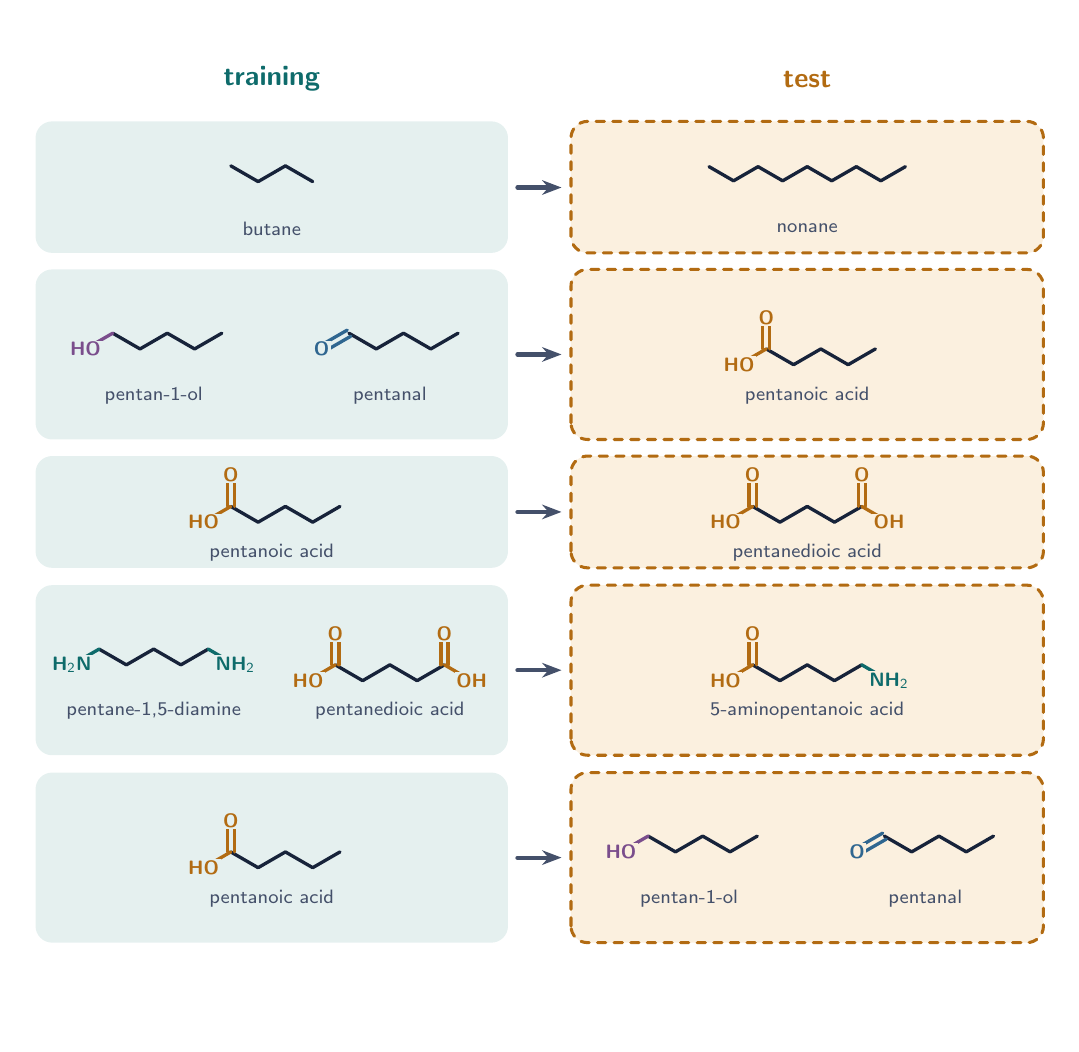
\begin{tikzpicture}
\useasboundingbox (-0.1,0.15) rectangle (12.9,-12.50);
\node[font=\bfseries, text=teal] at (3.0,-0.50) {training};
\node[font=\bfseries, text=amber] at (9.8,-0.50) {test};
\fill[tealsoft, rounded corners=6pt] (0.00,-2.71) rectangle (6.00,-1.04);
\draw[amber, dashed, line width=1.1pt, fill=ambersoft, rounded corners=6pt] (6.80,-2.71) rectangle (12.80,-1.04);
\draw[->, inksoft, line width=1.5pt] (6.12,-1.88) -- (6.68,-1.88);
\draw[ink, line width=1.2pt] (2.480,-1.605) -- (2.827,-1.805);
\draw[ink, line width=1.2pt] (2.827,-1.805) -- (3.173,-1.605);
\draw[ink, line width=1.2pt] (3.173,-1.605) -- (3.520,-1.805);
\node[font=\scriptsize, text=inksoft] at (3.00,-2.40) {butane};
\draw[ink, line width=1.2pt] (8.553,-1.615) -- (8.865,-1.795);
\draw[ink, line width=1.2pt] (8.865,-1.795) -- (9.176,-1.615);
\draw[ink, line width=1.2pt] (9.176,-1.615) -- (9.488,-1.795);
\draw[ink, line width=1.2pt] (9.488,-1.795) -- (9.800,-1.615);
\draw[ink, line width=1.2pt] (9.800,-1.615) -- (10.112,-1.795);
\draw[ink, line width=1.2pt] (10.112,-1.795) -- (10.424,-1.615);
\draw[ink, line width=1.2pt] (10.424,-1.615) -- (10.735,-1.795);
\draw[ink, line width=1.2pt] (10.735,-1.795) -- (11.047,-1.615);
\node[font=\scriptsize, text=inksoft] at (9.80,-2.40) {nonane};
\fill[tealsoft, rounded corners=6pt] (0.00,-5.08) rectangle (6.00,-2.92);
\draw[amber, dashed, line width=1.1pt, fill=ambersoft, rounded corners=6pt] (6.80,-5.08) rectangle (12.80,-2.92);
\draw[->, inksoft, line width=1.5pt] (6.12,-4.00) -- (6.68,-4.00);
\draw[ink, line width=1.2pt] (0.980,-3.730) -- (1.327,-3.930);
\draw[ink, line width=1.2pt] (1.327,-3.930) -- (1.673,-3.730);
\draw[ink, line width=1.2pt] (1.673,-3.730) -- (2.020,-3.930);
\draw[ink, line width=1.2pt] (2.020,-3.930) -- (2.366,-3.730);
\draw[plum, line width=1.2pt] (0.980,-3.730) -- (0.634,-3.930);
\node[font=\scriptsize\bfseries, text=plum, fill=tealsoft, inner sep=0.6pt] at (0.634,-3.930) {HO};
\node[font=\scriptsize, text=inksoft] at (1.50,-4.52) {pentan-1-ol};
\draw[ink, line width=1.2pt] (3.980,-3.730) -- (4.327,-3.930);
\draw[ink, line width=1.2pt] (4.327,-3.930) -- (4.673,-3.730);
\draw[ink, line width=1.2pt] (4.673,-3.730) -- (5.020,-3.930);
\draw[ink, line width=1.2pt] (5.020,-3.930) -- (5.366,-3.730);
\draw[blue, line width=1.2pt] (4.003,-3.769) -- (3.656,-3.969);
\draw[blue, line width=1.2pt] (3.958,-3.691) -- (3.611,-3.891);
\node[font=\scriptsize\bfseries, text=blue, fill=tealsoft, inner sep=0.6pt] at (3.634,-3.930) {O};
\node[font=\scriptsize, text=inksoft] at (4.50,-4.52) {pentanal};
\draw[ink, line width=1.2pt] (9.280,-3.930) -- (9.627,-4.130);
\draw[ink, line width=1.2pt] (9.627,-4.130) -- (9.973,-3.930);
\draw[ink, line width=1.2pt] (9.973,-3.930) -- (10.320,-4.130);
\draw[ink, line width=1.2pt] (10.320,-4.130) -- (10.666,-3.930);
\draw[amber, line width=1.2pt] (9.235,-3.930) -- (9.235,-3.530);
\draw[amber, line width=1.2pt] (9.325,-3.930) -- (9.325,-3.530);
\draw[amber, line width=1.2pt] (9.280,-3.930) -- (8.934,-4.130);
\node[font=\scriptsize\bfseries, text=amber, fill=ambersoft, inner sep=0.6pt] at (9.280,-3.530) {O};
\node[font=\scriptsize\bfseries, text=amber, fill=ambersoft, inner sep=0.6pt] at (8.934,-4.130) {HO};
\node[font=\scriptsize, text=inksoft] at (9.80,-4.52) {pentanoic acid};
\fill[tealsoft, rounded corners=6pt] (0.00,-6.71) rectangle (6.00,-5.29);
\draw[amber, dashed, line width=1.1pt, fill=ambersoft, rounded corners=6pt] (6.80,-6.71) rectangle (12.80,-5.29);
\draw[->, inksoft, line width=1.5pt] (6.12,-6.00) -- (6.68,-6.00);
\draw[ink, line width=1.2pt] (2.480,-5.930) -- (2.827,-6.130);
\draw[ink, line width=1.2pt] (2.827,-6.130) -- (3.173,-5.930);
\draw[ink, line width=1.2pt] (3.173,-5.930) -- (3.520,-6.130);
\draw[ink, line width=1.2pt] (3.520,-6.130) -- (3.866,-5.930);
\draw[amber, line width=1.2pt] (2.435,-5.930) -- (2.435,-5.530);
\draw[amber, line width=1.2pt] (2.525,-5.930) -- (2.525,-5.530);
\draw[amber, line width=1.2pt] (2.480,-5.930) -- (2.134,-6.130);
\node[font=\scriptsize\bfseries, text=amber, fill=tealsoft, inner sep=0.6pt] at (2.480,-5.530) {O};
\node[font=\scriptsize\bfseries, text=amber, fill=tealsoft, inner sep=0.6pt] at (2.134,-6.130) {HO};
\node[font=\scriptsize, text=inksoft] at (3.00,-6.52) {pentanoic acid};
\draw[ink, line width=1.2pt] (9.107,-5.930) -- (9.454,-6.130);
\draw[ink, line width=1.2pt] (9.454,-6.130) -- (9.800,-5.930);
\draw[ink, line width=1.2pt] (9.800,-5.930) -- (10.146,-6.130);
\draw[ink, line width=1.2pt] (10.146,-6.130) -- (10.493,-5.930);
\draw[amber, line width=1.2pt] (9.062,-5.930) -- (9.062,-5.530);
\draw[amber, line width=1.2pt] (9.152,-5.930) -- (9.152,-5.530);
\draw[amber, line width=1.2pt] (9.107,-5.930) -- (8.761,-6.130);
\draw[amber, line width=1.2pt] (10.448,-5.930) -- (10.448,-5.530);
\draw[amber, line width=1.2pt] (10.538,-5.930) -- (10.538,-5.530);
\draw[amber, line width=1.2pt] (10.493,-5.930) -- (10.839,-6.130);
\node[font=\scriptsize\bfseries, text=amber, fill=ambersoft, inner sep=0.6pt] at (9.107,-5.530) {O};
\node[font=\scriptsize\bfseries, text=amber, fill=ambersoft, inner sep=0.6pt] at (8.761,-6.130) {HO};
\node[font=\scriptsize\bfseries, text=amber, fill=ambersoft, inner sep=0.6pt] at (10.493,-5.530) {O};
\node[font=\scriptsize\bfseries, text=amber, fill=ambersoft, inner sep=0.6pt] at (10.839,-6.130) {OH};
\node[font=\scriptsize, text=inksoft] at (9.80,-6.52) {pentanedioic acid};
\fill[tealsoft, rounded corners=6pt] (0.00,-9.09) rectangle (6.00,-6.93);
\draw[amber, dashed, line width=1.1pt, fill=ambersoft, rounded corners=6pt] (6.80,-9.09) rectangle (12.80,-6.93);
\draw[->, inksoft, line width=1.5pt] (6.12,-8.01) -- (6.68,-8.01);
\draw[ink, line width=1.2pt] (0.807,-7.742) -- (1.154,-7.942);
\draw[ink, line width=1.2pt] (1.154,-7.942) -- (1.500,-7.742);
\draw[ink, line width=1.2pt] (1.500,-7.742) -- (1.846,-7.942);
\draw[ink, line width=1.2pt] (1.846,-7.942) -- (2.193,-7.742);
\draw[teal, line width=1.2pt] (0.807,-7.742) -- (0.461,-7.942);
\draw[teal, line width=1.2pt] (2.193,-7.742) -- (2.539,-7.942);
\node[font=\scriptsize\bfseries, text=teal, fill=tealsoft, inner sep=0.6pt] at (0.461,-7.942) {H$_2$N};
\node[font=\scriptsize\bfseries, text=teal, fill=tealsoft, inner sep=0.6pt] at (2.539,-7.942) {NH$_2$};
\node[font=\scriptsize, text=inksoft] at (1.50,-8.53) {pentane-1,5-diamine};
\draw[ink, line width=1.2pt] (3.807,-7.942) -- (4.154,-8.143);
\draw[ink, line width=1.2pt] (4.154,-8.143) -- (4.500,-7.942);
\draw[ink, line width=1.2pt] (4.500,-7.942) -- (4.846,-8.143);
\draw[ink, line width=1.2pt] (4.846,-8.143) -- (5.193,-7.942);
\draw[amber, line width=1.2pt] (3.762,-7.942) -- (3.762,-7.543);
\draw[amber, line width=1.2pt] (3.852,-7.942) -- (3.852,-7.543);
\draw[amber, line width=1.2pt] (3.807,-7.942) -- (3.461,-8.143);
\draw[amber, line width=1.2pt] (5.148,-7.942) -- (5.148,-7.543);
\draw[amber, line width=1.2pt] (5.238,-7.942) -- (5.238,-7.543);
\draw[amber, line width=1.2pt] (5.193,-7.942) -- (5.539,-8.143);
\node[font=\scriptsize\bfseries, text=amber, fill=tealsoft, inner sep=0.6pt] at (3.807,-7.543) {O};
\node[font=\scriptsize\bfseries, text=amber, fill=tealsoft, inner sep=0.6pt] at (3.461,-8.143) {HO};
\node[font=\scriptsize\bfseries, text=amber, fill=tealsoft, inner sep=0.6pt] at (5.193,-7.543) {O};
\node[font=\scriptsize\bfseries, text=amber, fill=tealsoft, inner sep=0.6pt] at (5.539,-8.143) {OH};
\node[font=\scriptsize, text=inksoft] at (4.50,-8.53) {pentanedioic acid};
\draw[ink, line width=1.2pt] (9.107,-7.942) -- (9.454,-8.143);
\draw[ink, line width=1.2pt] (9.454,-8.143) -- (9.800,-7.942);
\draw[ink, line width=1.2pt] (9.800,-7.942) -- (10.146,-8.143);
\draw[ink, line width=1.2pt] (10.146,-8.143) -- (10.493,-7.942);
\draw[amber, line width=1.2pt] (9.062,-7.942) -- (9.062,-7.543);
\draw[amber, line width=1.2pt] (9.152,-7.942) -- (9.152,-7.543);
\draw[amber, line width=1.2pt] (9.107,-7.942) -- (8.761,-8.143);
\draw[teal, line width=1.2pt] (10.493,-7.942) -- (10.839,-8.143);
\node[font=\scriptsize\bfseries, text=amber, fill=ambersoft, inner sep=0.6pt] at (9.107,-7.543) {O};
\node[font=\scriptsize\bfseries, text=amber, fill=ambersoft, inner sep=0.6pt] at (8.761,-8.143) {HO};
\node[font=\scriptsize\bfseries, text=teal, fill=ambersoft, inner sep=0.6pt] at (10.839,-8.143) {NH$_2$};
\node[font=\scriptsize, text=inksoft] at (9.80,-8.53) {5-aminopentanoic acid};
\fill[tealsoft, rounded corners=6pt] (0.00,-11.47) rectangle (6.00,-9.31);
\draw[amber, dashed, line width=1.1pt, fill=ambersoft, rounded corners=6pt] (6.80,-11.47) rectangle (12.80,-9.31);
\draw[->, inksoft, line width=1.5pt] (6.12,-10.39) -- (6.68,-10.39);
\draw[ink, line width=1.2pt] (2.480,-10.318) -- (2.827,-10.518);
\draw[ink, line width=1.2pt] (2.827,-10.518) -- (3.173,-10.318);
\draw[ink, line width=1.2pt] (3.173,-10.318) -- (3.520,-10.518);
\draw[ink, line width=1.2pt] (3.520,-10.518) -- (3.866,-10.318);
\draw[amber, line width=1.2pt] (2.435,-10.318) -- (2.435,-9.918);
\draw[amber, line width=1.2pt] (2.525,-10.318) -- (2.525,-9.918);
\draw[amber, line width=1.2pt] (2.480,-10.318) -- (2.134,-10.518);
\node[font=\scriptsize\bfseries, text=amber, fill=tealsoft, inner sep=0.6pt] at (2.480,-9.918) {O};
\node[font=\scriptsize\bfseries, text=amber, fill=tealsoft, inner sep=0.6pt] at (2.134,-10.518) {HO};
\node[font=\scriptsize, text=inksoft] at (3.00,-10.91) {pentanoic acid};
\draw[ink, line width=1.2pt] (7.780,-10.117) -- (8.127,-10.317);
\draw[ink, line width=1.2pt] (8.127,-10.317) -- (8.473,-10.117);
\draw[ink, line width=1.2pt] (8.473,-10.117) -- (8.820,-10.317);
\draw[ink, line width=1.2pt] (8.820,-10.317) -- (9.166,-10.117);
\draw[plum, line width=1.2pt] (7.780,-10.117) -- (7.434,-10.317);
\node[font=\scriptsize\bfseries, text=plum, fill=ambersoft, inner sep=0.6pt] at (7.434,-10.317) {HO};
\node[font=\scriptsize, text=inksoft] at (8.30,-10.91) {pentan-1-ol};
\draw[ink, line width=1.2pt] (10.780,-10.117) -- (11.127,-10.317);
\draw[ink, line width=1.2pt] (11.127,-10.317) -- (11.473,-10.117);
\draw[ink, line width=1.2pt] (11.473,-10.117) -- (11.820,-10.317);
\draw[ink, line width=1.2pt] (11.820,-10.317) -- (12.166,-10.117);
\draw[blue, line width=1.2pt] (10.803,-10.156) -- (10.456,-10.356);
\draw[blue, line width=1.2pt] (10.758,-10.079) -- (10.411,-10.279);
\node[font=\scriptsize\bfseries, text=blue, fill=ambersoft, inner sep=0.6pt] at (10.434,-10.317) {O};
\node[font=\scriptsize, text=inksoft] at (11.30,-10.91) {pentanal};
\end{tikzpicture}
\end{document}
